\section{Suggested solutions}

\subsection{Solution}

The figure \ref{fig:req_amount} shows the amount of requests and time that browser needs to make to generate a single VMO and  render a page. The browser needs to make more than 20 AJAX requests for a single page. The middleware was deployed on the local machine meaning that there is no latency bentween browser and middleware server. As can be seen, these are not optimistic numbers. The amount of requests is too high and computation have to be done on the both client and server sides. Several questions arises:
\begin{itemize}
	\item Is Redis a good caching layer for this project?
	\item Can Redis be replaced by something else? Maybe it would be better to use the configurational cache, represented by the web caches and control it through the http cache control headers.
\end{itemize}


\begin{figure}[h]
    \centering
	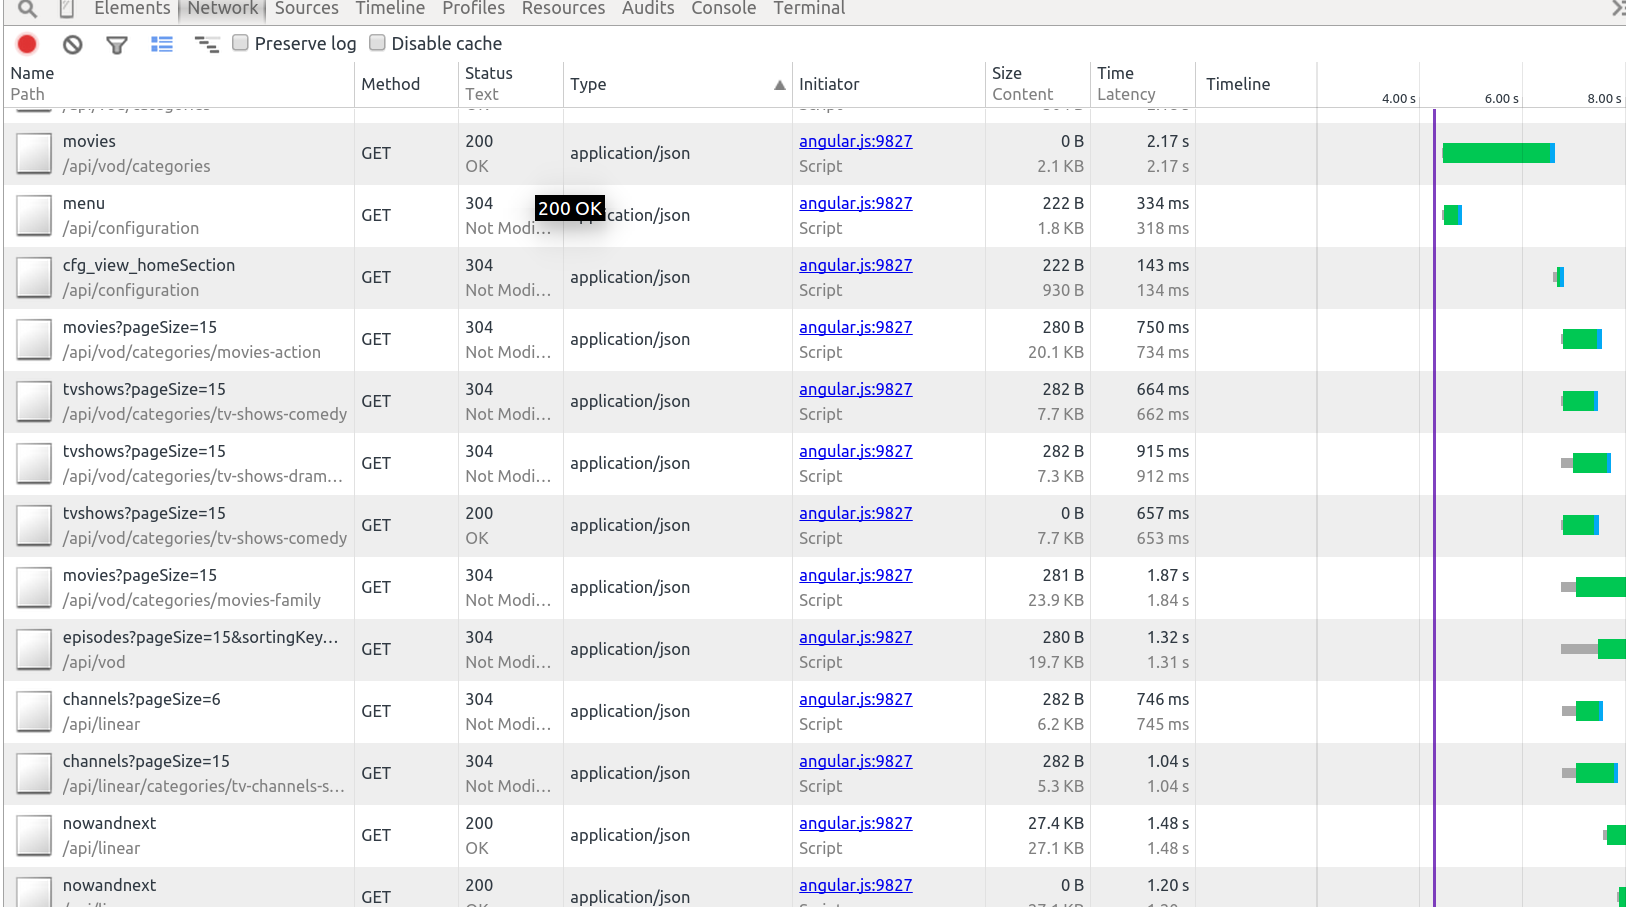
\includegraphics[width=\textwidth]{images/amount_of_requests.png}
    \caption{Example of page generation by browser}
    \label{fig:req_amount}
\end{figure}


The client application will make http requests through a reversed proxy server. The proxy sever will decide if the content is stale or not and will act as a web cache. The benefit of this solution is that instead of contacting server and than caching the object, the cache is contacted first and than the server. It theory it should give the performance and flexibility. The redis cache could be replaced by the Content Delivery Network solution in future. 

% describe your solution on the top level

\subsection{Web cache selection}

The web cache for the project should satisfy several parameters:
\begin{itemize}
	\item Configurable. The client application sends requests both for DMOs and for writing user actions. The web cache should not cache the requests for writing user actions. The sessions still should be supported in order to write user actions. 
	\item Responsive, easy maintanable. The web cache should be deployed easily and provide statistics and internal logging. 
	\item High performance. The web cache should be transparent and must not decrease the request time and latency if the cache object was not found locally. 
	% todo add more criterias
\end{itemize}

There are a many web cache solutions available both commertial and open source. For this project only open source solutions were considered. The initial candidates were: Squid, Varnish, Apache server with proxy module, Nginx server as a cachable reversed proxy and Apache Traffic Server.

The Squid server is a forward proxy server, but it can be configured as a reversed proxy server. Squid is preferably used for storing static content.

The Varnish was developed as a reversed proxy server from the beginning. It is fast, reliable and lightweigth. It uses Varnish Configuration Language(VCL) for configuration and describing the workflow. The VCL is translated to the C code and compiled to a shared object which is then dynamically linked into the server process. It is powerful tool that helps to set up Varnish as a dynamic reverse proxy server.

The Apache traffic server was developed by the Yahoo group and moved eventually to the Apache Incubator \cite{GuApacheTrafficUri}. According to Yahoo inc. Apache traffic server can handle more than 400TB of internet traffic per day and works as a forward as well as reversed proxy server. It has a growing community and continous improvement. The configuration is simple and consists of changing several files. All these, makes Apache traffic server a good candidate.  

Other solutions(Nginx and Apache server) was not developed to be a proxy servers, but have additional modules that one can install and configure. They are not well-configured and work worst than solutions described above \cite{GuApacheTrafficUri}[change].

The thorough comparison and performance evaluation could be found in \cite{VarnApacheReverse}.    

%TODO make a benchmarking analysis of the open web proxy caches
%TODO update the report, insert thate results about benchmarking and selection

\subsection{Web cache configuration}

Before performing execution and comparative study reversed proxy servers should be properly configured. They should aggregate and store requests that contain public data and skip analytical requests and requests with private user information(e.g. payments).

Proxy servers should also work with http sessions. Usually, when session is specified(the set-cookie http header included in the server response), proxy servers are transparent, meaning they are skipping these requests and not store them in memory. As was described in previous chapters, the metadata server uses http session for analytical purposes. It means that even anonymous users will have the unique session. 

In order to solve the problem, the Varnish replaces Cookie header with X-Cookie header. This gives the possibility for Varnish to store the requests and still have the analytical requests available. The metadata server was modified in order to treat X-Cookie header as a Cookie header.   

The Varnish configuration is presented in Appendix A.

\subsection{Testing tools}

In order to conduct necessary experiments the folowing tools were selected: Apache Benchmark tool and JMeter.

% Apache Benchmark tool serves as a lo 

JMeter is a tool that helps to measure the performance of applications that are using HTTP protocol. Jmeter was configured in order to simulate JSON and HTML requests that are required to render single page. The figure of Jmeter configuration is presented in Appendix B \ref{fig:jmeter_conf}. 
JMeter also builds the plot and the table of the request that was made with the corresponding time parameters.  

\subsection{Performance Comparison of Redis and Web caches}

% describe jmeter configuration

During the project several experiments were conducted. First, the figure [add figure of node.js jmeter] shows the results of executing JMeter script for existing company solution. The meaning of the columns is described below: 

\begin{itemize}
	\item Label  -- The name of the script that was executed
	\item Samles -- The amount of responses that was executed
	\item Average -- The average response time, represented in milliseconds
	\item Min -- the minimum time for the response 
	\item Max -- the maximum time for the response
	\item Std. Dev.  -- standard deviation from the average response time
	\item Error -- the persentage of error responses
	\item Throughput -- the throughput represented in responses per second
	\item KB/sec -- the data transferred per second
	\item Avg. Bytes -- the amount of bytes transferred per response
\end{itemize}

\subsection{View model objects}

% introduction
The company's solution was developed in order to provide flexibility and customisation to the end user. The middleware server retrieves all configuration from the metadata server. The configuration can be user specific information as well as global information e.g. the location of content distributors. The middleware translates the responses from the content distributors to Data Model Objects. They are the immutable objects that are transferred to the client's application. On the other hand, the client application operates with View Model Objects. They are used to reder HTML pages. Single HTML page can contain single View Model Object. The VMO is constructed from mutliple data model objects and some additional information(e.g. the location of the image).   

One important drawback could be noticed: application dublication. The middleware server and the client application have the same pattern of execution: they both operate with data and build new data patterns from existing ones. The difference is that the middleware server is doing it with content distributor responses and the client aplication is processing middleware responses. Because of this situation, the client application should make several HTTP requests for retrieving necessary DMO objects from the middleware server.  The example of the single page generation is on the picture [put picture]. As can be seen, in order to generate a single main page, the client application has to make about 10 Ajax requests. What, if there was a possibility to generate the VMO objects on the middleware side?  Maybe, there would be a possibility to get rid of the dublication? What should be done for it? This section will answer these questions.

\subsubsection{VMO properties}

% describe examination of applications(Algar, RTelecom, ViaWeb)

Typical DMO and VMO objects are presented in appendix C[Add appendix C]. As could be seen a VMO object is a JSON dictionary build from DMO objects. Lets define the set of properties that VMO supports:

Generic. The DMO objects are specific and unique for every content distributor. They are build according to the specific rules in the middleware server. The VMOs are generated from DMOs according to another set of rules specified in the client application. As a result in order to move VMO generation to the server side some descriptive language should be introduced that lets developers to describe the VMO structure.

Hierarchical. DMOs are basically data from content distributors. That means that the DMOs can be depend on other DMOs. For example, the figure [add DMO dep. figure] shows that in order to build a movie list DMO, first the DMO that represents movie categories should be generated, than for each movie category, the set of movie objects should be fetched, and only on the third step, the list of movies could be build. These means that the VMOs have a hierarchical structure. The typical VMO is presented on picture [figure of VMO]. 

\subsubsection{New Middleware server architecture}

In the current architecture, the single instance of the middleware server is deployed for a single content distributor. This is done due to the specifics of content distributors and data that they are providing. The question arises, is there a possibility to move the individual logic that requires to processes data to the client application while keeping the middleware as generic as possible? The theoretical benefits of this approach are: there will be needed single middleware server or cluster deployed. It will simplify the deploying system: instead of supporting middleware for every content distributor, there will be just one. The new architecture is presented of figure \ref{fig:arch_overview_new}. As can be seen, the configuration server(Appgrid) is now treated like a content distributor. The benefit is that we do not need specify separate logic for it. 

\begin{figure}[h]
    \centering
	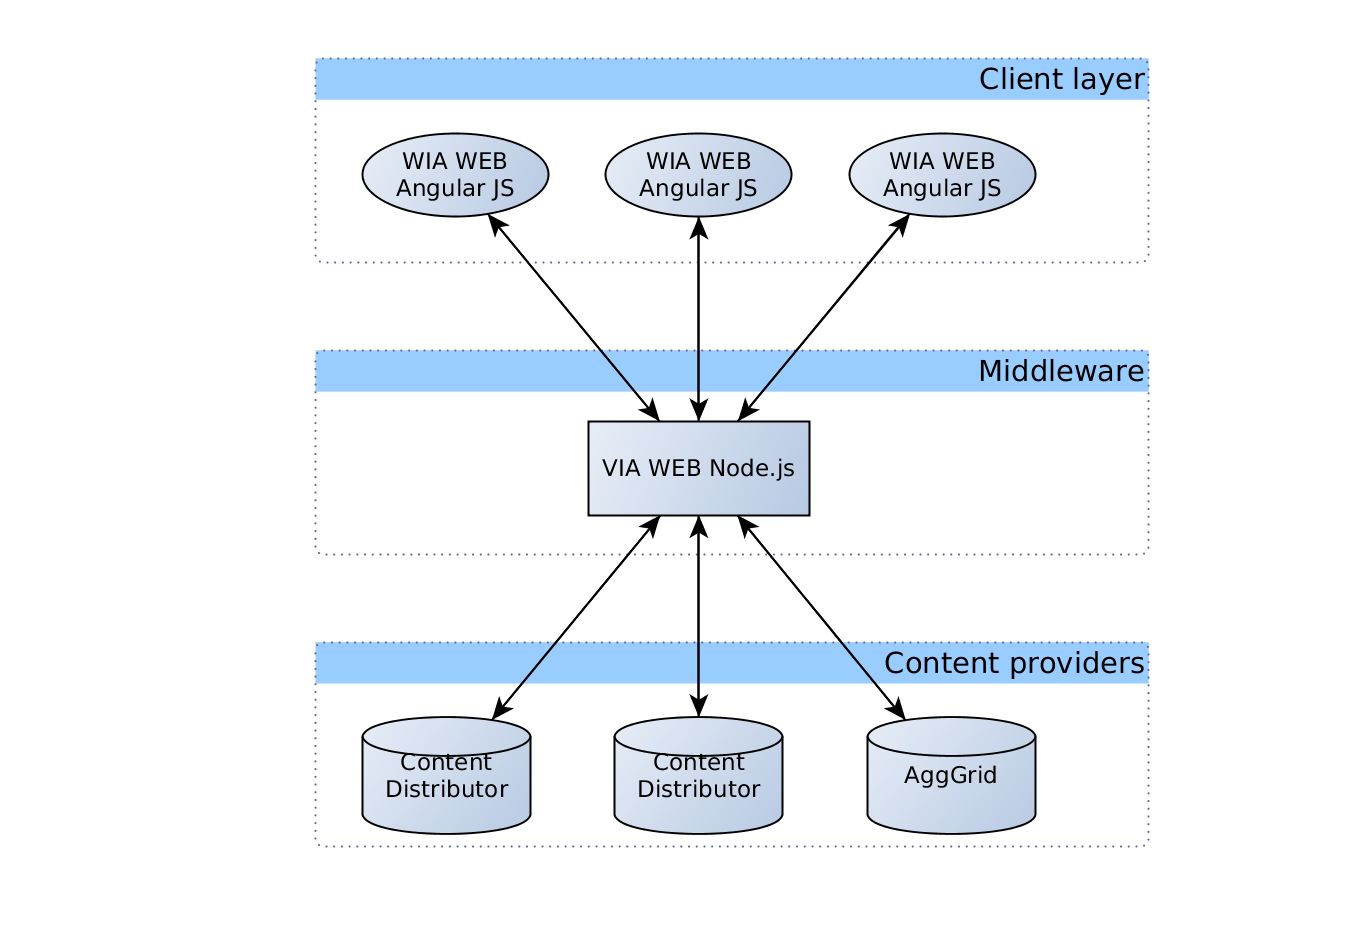
\includegraphics[width=\textwidth]{images/thesis_global_architecture_new.png}
    \caption{Manager workflow}
    \label{fig:arch_overview_new}
\end{figure}

Lets abstract from the architecture and look at the middleware server from the abstarct point of view.
The middleware server receives queries for the VMO generation. It supporsts several content distributors(databases), it makes queries to the content distributors for retrieving data model objects(tables). The middleware server resembles a lot a relational database system. The comparison of database management system and middleware server:

\begin{center}
  \begin{tabular}{||p{3in}|||p{3in}||}
    \hline
    Database & Middleware server VMO generation  \\ \hline
    serves multiple clients & should serve multiple client applications  \\ \hline
    supports creation of new databases & should support insertion of new content servers  \\ \hline
    supporst creation and alternation of tables & should support creation and alternation of new endpoints  \\ \hline
    supports dynamic queries to the desired databases and tables & should support queries to the content distributors and theis endpoints \\ \hline
    \hline
  \end{tabular}
\end{center}

\subsubsection{Approach description}

Let's consider relational database management systems and applications that are using them. There is usually a single instance or cluster of databases insalled and deployed on servers, depending on the amount of requests it should serve. Nobody makes new database instance for a single client, because it is neither efficient nor effective. In order to get data from the database the queiries are executed. The SQL queries are basically the rich descriptive language that is interpreted by the database and executed for specified tables. The data is provided in two forms: array of table rows and array of view rows. Tables are the single source of information that resembles a lot DMO. Views are the mixed information from tables that looks like VMO. 

In order to solve the problem of dublication and reduce the amount of requests, the hierarchical VMO generator(HVG) was developed. The HVG basicaclly the descriptive language, that developers are writing in a JSON format. The json is then translated into the GET HTTP or POST HTTP request and sended  to the middleware server. The middleware server parses the request, builds the asyclic graph and fetches the corresponding data model objects. The data model objects then combined together and sended as a response to the client application. The client application executes specific logic on the data received from server and builds HTML pages.

% The picture [insert picture] describes the VMO 

% picture of DBMS and Middleware server
% picture of DBMS tables and queries to the middleware server

\subsubsection{Path in VMOs}

This section introduces the definition of path in the View Modelw Object. The main format for data transferring is JSON. The JSON format consists of two main objects: array and dictionary. The example of dictionary: 
% {key:value}
The example of array: 
% [value1,value2]
Very complicated entities can be built using combinations of these two objects. Let's introduce the definition of path: The path is the route to the specific object or a set of objects in a JSON entity. 
The examples of path is presented of figure[add figure]. 

The path identifies single object if it lays though a set of dictionaries. However, if the array is found, all elements will be traversed and a set of corresponding objects will be extracted. 

\subsubsection{Hierarchical VMO Generator}

In order to solve the problem of multiple requests and middleware server dublication, the descriptive hierarchical VMO generator was implemented. It consists of three parts: content provider dictionary, queries and parser. 

The content provider dictionary has a tree based structure and its scheme is presented on \ref{fig:content_provider_map}. The rectangles indicate the single instance of object and the parallelograms indicate the dictionary of objects. The content provider dictionary contains a dictionary of content providers. Each content provider consitst of two parts: location and a dictionary of resources. The location in a domain with corresponding scheme. The resource has one field: endpoint. The endpoint is a path in URI[RFC to URI] with embedded templates. The template can be one of two types: \textit{\{param\_id\}} and \textit{\{param\_id*\}}. The first type indicates that only one value can replace the template. If array of values is given, it will produce the array of resolved endpoints. On the other hand, the second type produces single endpoint, even if array of values is given. The examples of templates are presented below: 

% TODO: purpose

\begin{center}
  \begin{tabular}{l l}
    Input values: & \textit{\{id:[value1,value2,value3]\}} \\
    Endpoint: & \textit{http://testdomain.ext/\{id\}}  \\ 
    Result: & [\textit{http://testdomain.ext/value1}   \\
    		&  \textit{http://testdomain.ext/value2}   \\
    		&  \textit{http://testdomain.ext/value3}]  \\
    Endpoint: & \textit{http://testdomain.ext/\{id*\}} \\
    Result: &  \textit{http://testdomain.ext/value1,value2,value3}
  \end{tabular}
\end{center}

The example of content provider map is given in Appendix C.


\begin{figure}[h]
    \centering
	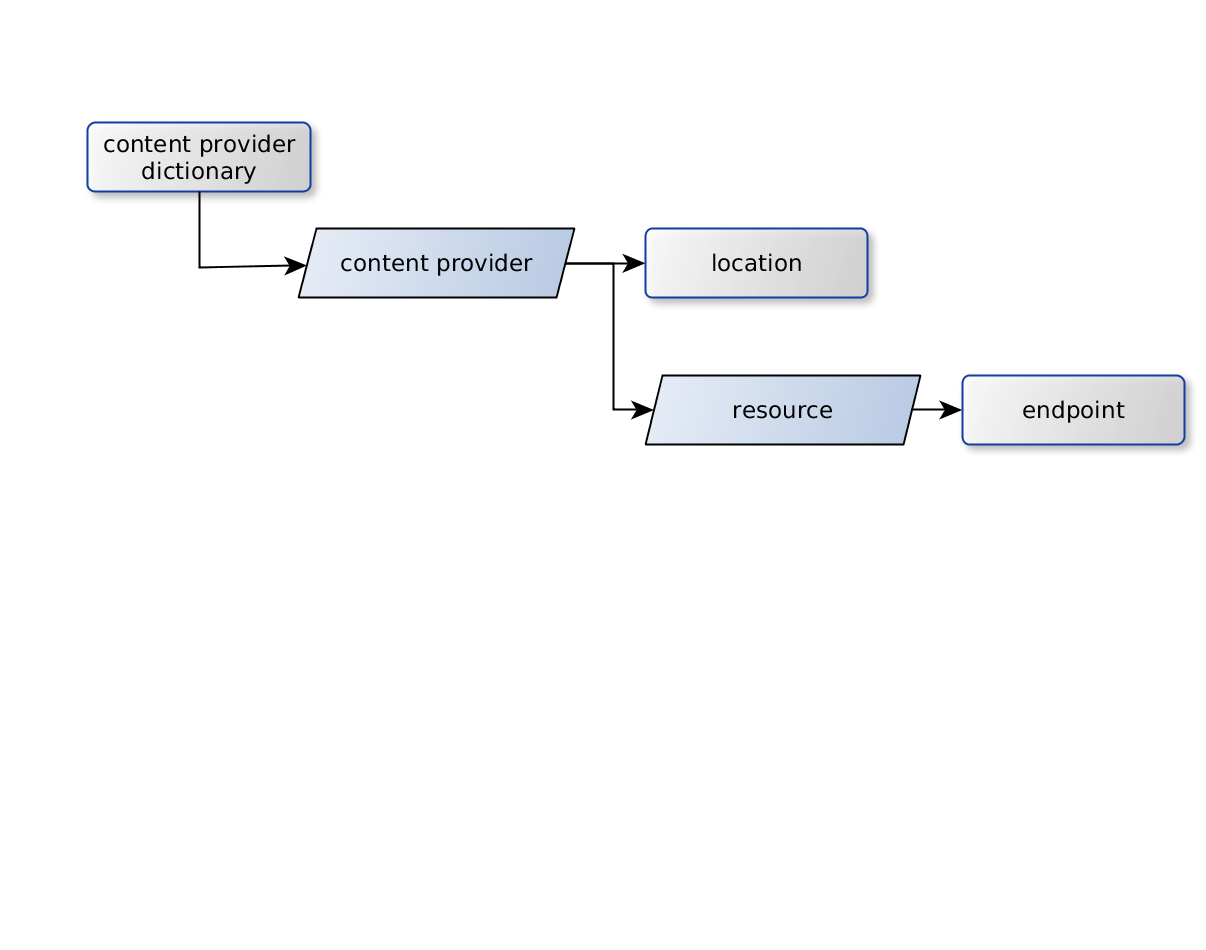
\includegraphics[width=\textwidth]{images/content_provider_map.png}
    \caption{Content Provider dictionary structure}
    \label{fig:content_provider_map}
\end{figure}


They query represents the request from the client application to the middleware server. The tree based structure is presented on figure \ref{fig:query_structure}. The query consists of several query objects.
Each query object may have up to three parameters: \textit{content\_distributor}, \textit{path\_parameters}, \textit{query\_parameters}. The content distributor corresponds to the key in content provider dictionary desrcibed above. Through it the set of resources is retrieved from the content provider dictionary. The \textit{path\_parameters} and \textit{query\_parameters} have the similar structure, as a result only one of them will be described.The \textit{path\_parameters} is a dictionary of parameters, the key corresponds to the template parameter in resource object described above. Each \textit{path\_parameter} has type field. It can have one of two values: \textit{constant} or \textit{dependency}. If the value is \textit{constant}, only one additional field should be specified: \textit{values}. This field serves as a container of values that should replace the corresponding template in the endpoint. 

On the other hand, if the value is \textit{dependency} the query object depends on another query object e.g. for getting the list of movies from the content distributor, the list of categories should be requested first. In this case, additional parameters should be specified: \textit{parent}, \textit{parent\_parameter\_type}, \textit{path}, \textit{property}.    


\begin{figure}[h]
    \centering
	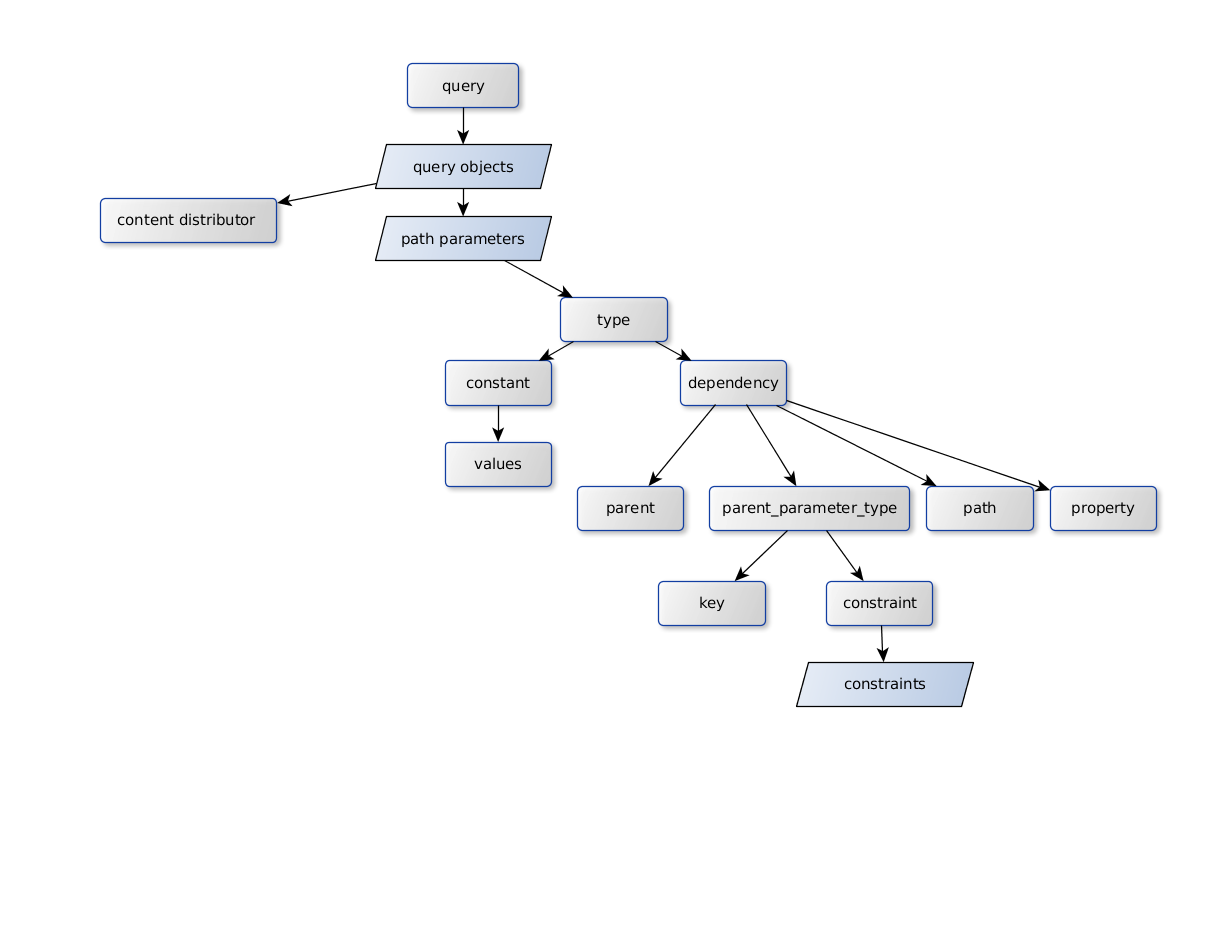
\includegraphics[width=\textwidth]{images/query_structure.png}
    \caption{Query structure}
    \label{fig:query_structure}
\end{figure}


\subsubsection{JSON language description}

The JSON HVG request is a dictionary with one or several objects. The objects describe the resource requests with specified parameters. The key in dictionary is an identifier of requested object. The value is a dictionary represeting the set of parameters. 
The description of fields is presented in table below: [add table];

The \textit{content\_distributor} field represents the content provider from which the data will be gathered.

The path\_parameters: the dictionary of path parameters. Every path parameter corresponds to the path parameter in the urlTempalte field that was described in previous section. When the request is executed, the parameters in urlTemplate field would be changed to the parameters indecated in this field. 
The key in the path\_parameters dictionary is a id that identifies the place in urlTemplate field.
The value is a dictionary that describes the parameter. 
The type can be constant or dependency. The parameter that have consant type should have mandatory field values that represents the array of values. 

\subsubsection{Architecture of VMOs}

% how they are working, what did you change and introduce 
% describe what changes did you make in order to make vmos work


\subsubsection{Comparison}

% teoreticaly compare current dmos, vmos and amos(application model objects)

